\documentclass{beamer}
%\usetheme{Ilmenau}
%\usecolortheme{beaver}

\usepackage[slovak,american]{babel}
\usepackage[utf8]{inputenc}
\usepackage{graphicx}
\usepackage{adjustbox}
 \usepackage{xcolor}
 
 \newsavebox\MBox
\newcommand\Cline[2][red]{{\sbox\MBox{$#2$}%
  \rlap{\usebox\MBox}\color{#1}\rule[-2.2\dp\MBox]{\wd\MBox}{1pt}}}

%\usefonttheme{serif}

\definecolor{UKOrange}{HTML}{ef9424} %
\definecolor{UKBrown}{HTML}{a96d5e} %
\definecolor{UKLight}{HTML}{d8b6ab} %
\definecolor{UKDark}{HTML}{7a4f44}
\definecolor{UKDarker}{HTML}{4d312b} 
\definecolor{UKDarkest}{HTML}{2e1e1a}
\definecolor{UKRed}{HTML}{bf1f1c}

\setbeamertemplate{footline}[frame number]{}
\setbeamertemplate{navigation symbols}{}

%\usecolortheme{beaver}
\setbeamertemplate{itemize item}[square]
\setbeamercolor{itemize item}{fg = UKBrown}
\setbeamercolor{itemize subitem}{fg = UKLight}
\setbeamercolor{enumerate item}{fg = UKDark}

\setbeamercolor{footnote}{fg=UKLight}
\setbeamercolor{footnote mark}{fg=UKLight}
\setbeamerfont{footnote}{size=\tiny}
\renewcommand\footnoterule{}

\usetheme{default}
\beamertemplatenavigationsymbolsempty
\setbeamercolor{title}{fg=white, bg=UKBrown}
\setbeamercolor{frametitle}{fg=white, bg=UKBrown}
\setbeamercolor{block title}{bg=UKBrown, fg= white}
\setbeamercolor{block body}{bg =UKLight, fg = UKDarkest}

\useoutertheme[subsection=false]{miniframes}
\AtBeginSection[]{\subsection{}}

\setbeamercolor{below lower separation line head}{bg=UKDark}
\addtobeamertemplate{headline}{}{%
  \begin{beamercolorbox}[colsep=0.5pt]{below lower separation line head}
  \end{beamercolorbox}
}
%\setbeamercolor*{mini frame}{fg=white,bg=UKRosy}
\setbeamercolor{section in head/foot}{fg=UKLight, bg=UKDark}

%\setbeamertemplate{itemize/enumerate body begin}{\normalsize}
%\setbeamertemplate{itemize/enumerate subbody begin}{\normalsize}




%\newcommand{\codeblock}[2]{ \begin{block}{#1} \begin{verbatim}#2\end{verbatim}\end{block}}

%\defbeamertemplate*{title page}{customized}[1][]
%{
%  \begin{centering}
%    \begin{beamercolorbox}[sep=8pt,center]{title}
%      \usebeamerfont{title}\inserttitle
%    \end{beamercolorbox}
%  \end{centering}
%  \bigskip
%
%\begin{columns}[onlytextwidth,T]
%
%
%  \column{27mm}
%  \includegraphics[width=27mm]{images/logoFMFI.png}
%  
%  \column{\dimexpr\linewidth-54mm-6mm}
%  \centering
%  \vspace{5mm}  
%  \usebeamerfont{author}\insertauthor\par
%  \vspace{5mm}
%  \usebeamerfont{institute}\insertinstitute\par
%
%  \column{27mm}
%  \includegraphics[width=27mm]{images/logoUK.png}  
%\end{columns}
%\centering
%\vspace{7mm}
%  \usebeamerfont{date}\insertdate\par
%}


\title[PCA a LDA]{Rozpoznávanie obrazcov - 6. cvičenie \\ Lineárny klasifikátor a SVM}
\author[Viktor Kocur]{Viktor Kocur \\{\small viktor.kocur@fmph.uniba.sk}}
\institute{DAI FMFI UK}
\date{30.3.2020}
%\titlegraphic{\includegraphics[width=2.7cm]{images/logoFMFI.png}\hspace*{1cm}~%
%   \includegraphics[width=2.7cm]{images/logoUK.png}
%}


\begin{document}
\selectlanguage{slovak}

\begin{frame}[plain]
  \titlepage  
\end{frame}

\section{Lineárny klasifikátor}

\begin{frame}
\frametitle{Lineárny klasifikátor}
\begin{block}{Základný princíp}
Jadrom lineárneho klasifikátora je lineárna funkcia $f : \mathbb{R}^n \mapsto \mathbb{R}, f(\vec{x}) = \vec{w}^T \vec{x} + b$, kde $\vec{x}$ je príznakový vektor, $\vec{w}$ je vektor váh a $b$ je tzv. bias člen.
\end{block}

\begin{block}{Klasifikácia}
Ak máme dve triedy $\omega_1$ a $\omega_2$, tak príznakový vektor $\vec{x}$ priradíme do triedy $\omega_1$ ak $f(\vec{x}) \ge 0$, do triedy $\omega_2$ ak $f(\vec{x}) < 0$.
\end{block}
\end{frame}



\begin{frame}
\frametitle{Lineárny klasifikátor}
\begin{block}{Geometrický význam}
Funkcia $f$ v skutošti delí príznakový priestor na dve časti oddelené nadrovinou. Body pre ktoré $f(\vec{x}) = 0$ ležia práve na tejto nadrovine. 
\end{block}

\begin{block}{Cieľ trénovania}
Pri tréningu teda chceme nájsť také parametre, aby nadrovina, ktorú využívame rozdelovala trénovaciu množinu čo najlepšie.
\end{block}
\end{frame}


\begin{frame}
\frametitle{Lineárny klasifikátor}
\center
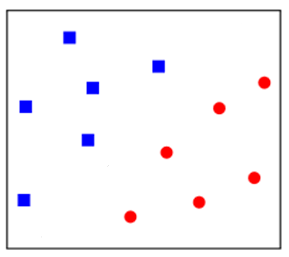
\includegraphics[width=0.8\textwidth]{lc1.png}
\end{frame}


\begin{frame}
\frametitle{Lineárny klasifikátor}
\center
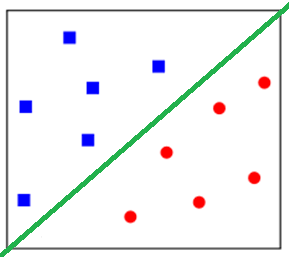
\includegraphics[width=0.8\textwidth]{lc2.png}
\end{frame}

\begin{frame}
\frametitle{Trénovanie}
\begin{block}{Trénovacie dáta}
Na natrénovanie klasifikátora budeme potrebovať tzv. trénovacie dáta. Teda ku vektoru $\vec{x}$ potrebujeme označenie triedy $y \in \{0,1\}$. Náš cieľ je aby náš klasifikátor fungoval dobre na trénovacích dátach. 
\end{block}

\begin{block}{Regularizácia}
Niekedy chceme klasifikátor, ktorý nieje najlpší na trénovacích dátach ale vie dobre generaliozovať. To sa nazýva regularizácia.
\end{block}

\begin{block}{Cenová funkcia}
Dobrý klasifikátor dostaneme tak, že vyvtvoríme tzv. cenovú funkciu $C : \mathbb{R}^{n+1} \mapsto \mathbb{R}, C(b, \vec{w})$, ktorá má globálne minimum pre také parametre ktoré rozdelujú triedy čo najlepšie. Trénovanie je potom vlastne optimalizačná úloha.
\end{block}
\end{frame}

\begin{frame}
\frametitle{Cenová funkcia - I}
\begin{block}{Zjednodušenie}
Keďže člen $b$ je nám to to trocha komplikuje, tak zavedieme nové značenie: $\vec{\theta} = (b, \vec{w})$ a ako vektor $\vec{X} = (1, \vec{x})$. Toto nám umožní zapísať $f(\vec{X}) = \vec{\theta}^T \vec{X}$.
\end{block}

\begin{block}{Sigmoid}
Pri definícii použijeme sigmoidálnu funkciu: $\sigma(z) = \frac{1}{1+e^{-z}}$.
\end{block}

\begin{block}{Sigmoid - derívacia}
$\sigma(z)' = \sigma(z) (1 - \sigma(z))$.
\end{block}
\end{frame}


\begin{frame}
\frametitle{Sigmoid}
\center
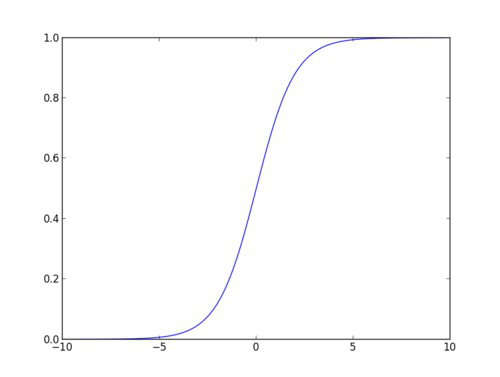
\includegraphics[width=0.8\textwidth]{sigmoid.png}
\end{frame}



\begin{frame}
\frametitle{Cenová funkcia - II}
\begin{block}{Zjednodušenie}
Zavedieme ešte jednu funkciu: $h_{\theta} = \sigma(f(\vec{x}))$.
\end{block}

\begin{block}{Cenová funkcia - binary crossentropy}
\begin{equation*}
J(\vec{\theta}) = \frac{1}{m} \sum_{i=1}^m \left( -y^{(i)} log(h_{\theta}(\vec{x}^{(i)})) - (1 - y^{(i)}) log(1 - h_{\theta} (\vec{x}^{(i)})) \right)
\end{equation*}
\end{block}

\begin{block}{Cenová funkcia - derívacia}
\begin{equation*}
\frac{\partial J}{\partial \theta_j} = \frac{1}{m} \sum_{i=1}^m \left( h_{\theta}(\vec{x}^{(i)}) - y^{(i)} \right) x_j^{(i)}
\end{equation*}
\end{block}
\end{frame}


\begin{frame}
\frametitle{Optimalizácia}
\begin{block}{Gradientný zostup}
$\theta_i := \theta_i - \eta \frac{\partial J}{\partial \theta_i}$
\end{block}

\begin{block}{Skutočná optimalizácia}
V skutočnosti sa používajú sofistikovanejšie algoritmy. Ako napríklad SGD, alebo metódy založené na Hessovej matici.
\end{block}

\begin{block}{Optimalizácia v matlabe}
x = fminunc(fun,x0) - nájde optimálne parametre x pre ktoré je funkcia fun minimálna (ak sa to podarí). Keďže sa používajú iteratívne metódy, tak je nutné zadať inicializačné hodnoty x0.
\end{block}
\end{frame}

\begin{frame}
\frametitle{Optimalizácia}
\begin{block}{Úloha}
Prezrite si skript LinearClassifier.m
\end{block}

\begin{block}{Úloha}
Dokončite funkciu costFunction. Pomocou cenovej funkcie ktorá je na pár slidoch dozadu.
\end{block}
\end{frame}



\begin{frame}
\frametitle{Lineárny klasifikátor - Matlab}
\begin{block}{Regularizácia}
K cenovej funkcii pridáme aj regularizačný člen: $C_R(\vec{\theta}) = C(\vec{\theta}) + R(\vec{\theta})$. Napríklad $R(\vec{\theta}) = \sum_{i=2}^n \theta_i^2$, alebo $\sum_{i=2}^n |\theta_i |$
\end{block}


\begin{block}{fitclinear}
Mdl = fitclinear(x,y) - vráti lineárny klasifikačný model Mdl pre príznakové vektory ktoré su riadkami matice x a k nim korešpondujúcimi triedami y. Táto funkcia dokáže aj SVM aj logistickú regresiu. Pre možnosti sa pozrite do helpu. Defualtne sa tu využíva aj regularizácia.
\end{block}

\begin{block}{Mdl.predict}
Mdl.predict(x) - vráti triedu pre daný príznakový vektor.
\end{block}
\end{frame}


\begin{frame}
\frametitle{Lineárny klasifikátor - Matlab}
\begin{block}{Mdl.Beta, Mdl.Bias}
Mdl.Beta - vráti to čo sme si označovali ako vektor $\vec{w}$. Mdl.Bias - vráti to čo sme si označili ako $b$.
\end{block}


\begin{block}{Úloha}
Do obrázku (gscatter) s dátami z ex2data1.txt dokreslite delaicu priamku pre klasifikátor z fitclinear. Môžete použiť plot, alebo refline. Pozn.: pre refline použijeme:
$$\beta_1 \cdot x_1 + \beta_2 \cdot x_2 + bias = 0 \iff  x_2 = m \cdot x_1 + b $$
$$x_2 = -\frac{\beta_1}{\beta_2} \cdot x_1 - \frac{bias}{\beta_2}$$
$$ m = -\frac{\beta_1}{\beta_2}, b = - \frac{bias}{\beta_2}$$
\end{block}
\end{frame}

\section{SVM}

\begin{frame}
\frametitle{Princíp}
\center
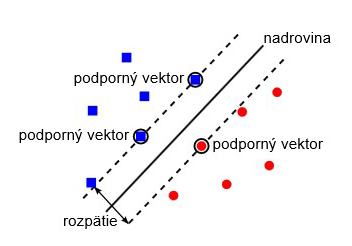
\includegraphics[width=0.8\textwidth]{svm.png}
\end{frame}

\begin{frame}
\frametitle{SVM}
\begin{block}{Princíp}
SVM nájde podporné vektory a snaží sa nájsť deliacu čiaru tak, aby bolo rozdelovací pás čo najširší pomocou podmienky pre podporné vektory vo forme $\vec{w}^T \vec{x} + b = \pm 1$.
\end{block}

\begin{block}{Kernelový trik}
Dáta často niesu lineárne separabilné. Preto je nutné príznakový priestor transformovať pomocou tzv. kernelu. Teda funkcie $\phi : \mathbb{R}^n \mapsto \mathbb{R}^{m}$, pre ktorú platí, že existuje funkcia $k$, tž: $k(x_i, x_j) = \phi(x_i) \phi(x_j).$ SVM potom hľadá lineárny klasifikátor v novom priestore $\mathbb{R}^m$. 
\end{block}
\end{frame}


\begin{frame}
\frametitle{SVM}
\begin{block}{fitcsvm}
SVMMdl = fitcsvm(X,y) - vráti SVM model natrénovaný na príznakoch X a triedach y.
\end{block}

\begin{block}{fitcsvm}
SVMMdl = fitcsvm(X,y, 'KernelFunction',nazov, 'KernelScale', 'auto') - vráti SVM s kernelovým trikom. Pozor nezabudnite na KernelScale.
\end{block}
\end{frame}


\begin{frame}
\frametitle{SVM - Úloha}
\begin{block}{showSVM}
showSVM(SVMMdl, X, y) - zobrazí SVM model pre 2D dáta X, y (je to .m file v zipe)
\end{block}

\begin{block}{Úloha}
Zobrazte si SVM s rôznymi kernelmi. Skúste čo sa stane ak nenastavíte KernelScale.
\end{block}
\end{frame}

\end{document}